\section{2-trees}
A new family of graphs is investigated for its edge-length ratio optimization on a fixed grid. A $k$-tree is an undirected graph which is incrementally created from a $K_{k+1}$ in a way that each added vertex has exactly $k$ neighbours such that those $k+1$ vertices form a clique. Following this definition, a $4$-tree is not planar since it starts with a $K_5$. Of interest is the 2-tree. \\
Since the class of 2-trees correspond to the class of maximal series-parallel graphs (\cite{DBLP:journals/corr/abs-2108-12628}, Page 2), a drawing algorithm by Biedl for SP-graphs is modfied to minimize the edge-length ratio. 

\subsection{Previous results}

There are several results for small planar drawings of outerplanar and series-parallel graphs. Among others, it was shown that:
\begin{itemize}
	\item Every series-parallel graph has a visibility representation with $\mathcal{O}(n^{\frac{3}{2}})$ area
	\item Every series-parallel graph has a visibility representation with $\mathcal{O}(\Delta n\log n)$ area, where $\Delta$ is the maximum degree of the graph
	\item It was reproven that every outerplanar graph is series-parallel, therefore these results also apply for outerplanar graphs [\cite{DBLP:journals/dcg/Biedl11}: Page 2,3]
\end{itemize}
Visibility respresentations and orthogonal drawings can be converted to poly-line drawings. The following relationships hold for drawing models:
\begin{description}
	\item[Visibility Representation] Vertices are boxes, edges are horizontal or vertical line segnemts. In a 1-directional visibility representation all edges are vertical line segments.
	\item[Orthogonal Box-Drawing] Vertices are axis-aligned boxes (possibly degenerated to a line segment or point) and edges are sequences of contiguous horizontal or vertical line segments. A 1-directional visibility representation is also automatically an orthogonal box-drawing. In a flat orthogonal box drawing, every vertex is a vertical line segment.
	\item[Poly-line drawing] Vertices are points, edges are sequences of contiguous straight-line segments. A transition point between two straight-line segments is called a bend. A poly-line drawing can be obtained by modifying an orthogonal box drawing in a way such that a vertex is reassigned to a point inside of the prior box and the incident edges are rerouted to this very point. Also, empty grid lines are added until every edge has length at least 2. The area consumption is asymptotically the same since the width and height is doubled at most.
	[\cite{DBLP:journals/dcg/Biedl11}: Page 5,6]
\end{description}
Since visibility representations and orthogonal box drawings can be converted to polyline drawings with asymptotically the same area, the upper bounds given for the visibility representation also hold for poly-line drawings.
\subsection{The drawing algorithm for a maximal series-parallel graph}
The drawing algorithm creates a visibility representation of a given maximal series-parallel graph and is also defined recursively based on 2-terminal SP graphs. The maximum height of the drawing is given by a recursive formula, depending of the heights of the subgraphs. [\cite{DBLP:journals/dcg/Biedl11}: Page 6 to 11]
Concerning the edge-length ratio, the longest edge might depend on the height of the drawing while the shortest edge might be of unit length. The upper bound for the height will be determined with help of a recursive function $h(m)$, where $m$ describes the amount of edges.
\begin{description}
	\item[Invariant] Vertex $s$ contains the upper right corner of the bounding box, while vertex $t$ contains the lower right corner of the bounding box. The boxes for $s$ and $t$ can be stretched to the whole width of the drawing.
	\item[Base case] the base case is the edge $(s,t)$. Simply put $s$ over $t$ and the invariant holds. Here, the recursive function for the height description stops at $h(1) = 2$.
		\begin{figure}[H]
		\centering
		\begin{subfigure}{0.3\linewidth}
			\centering
			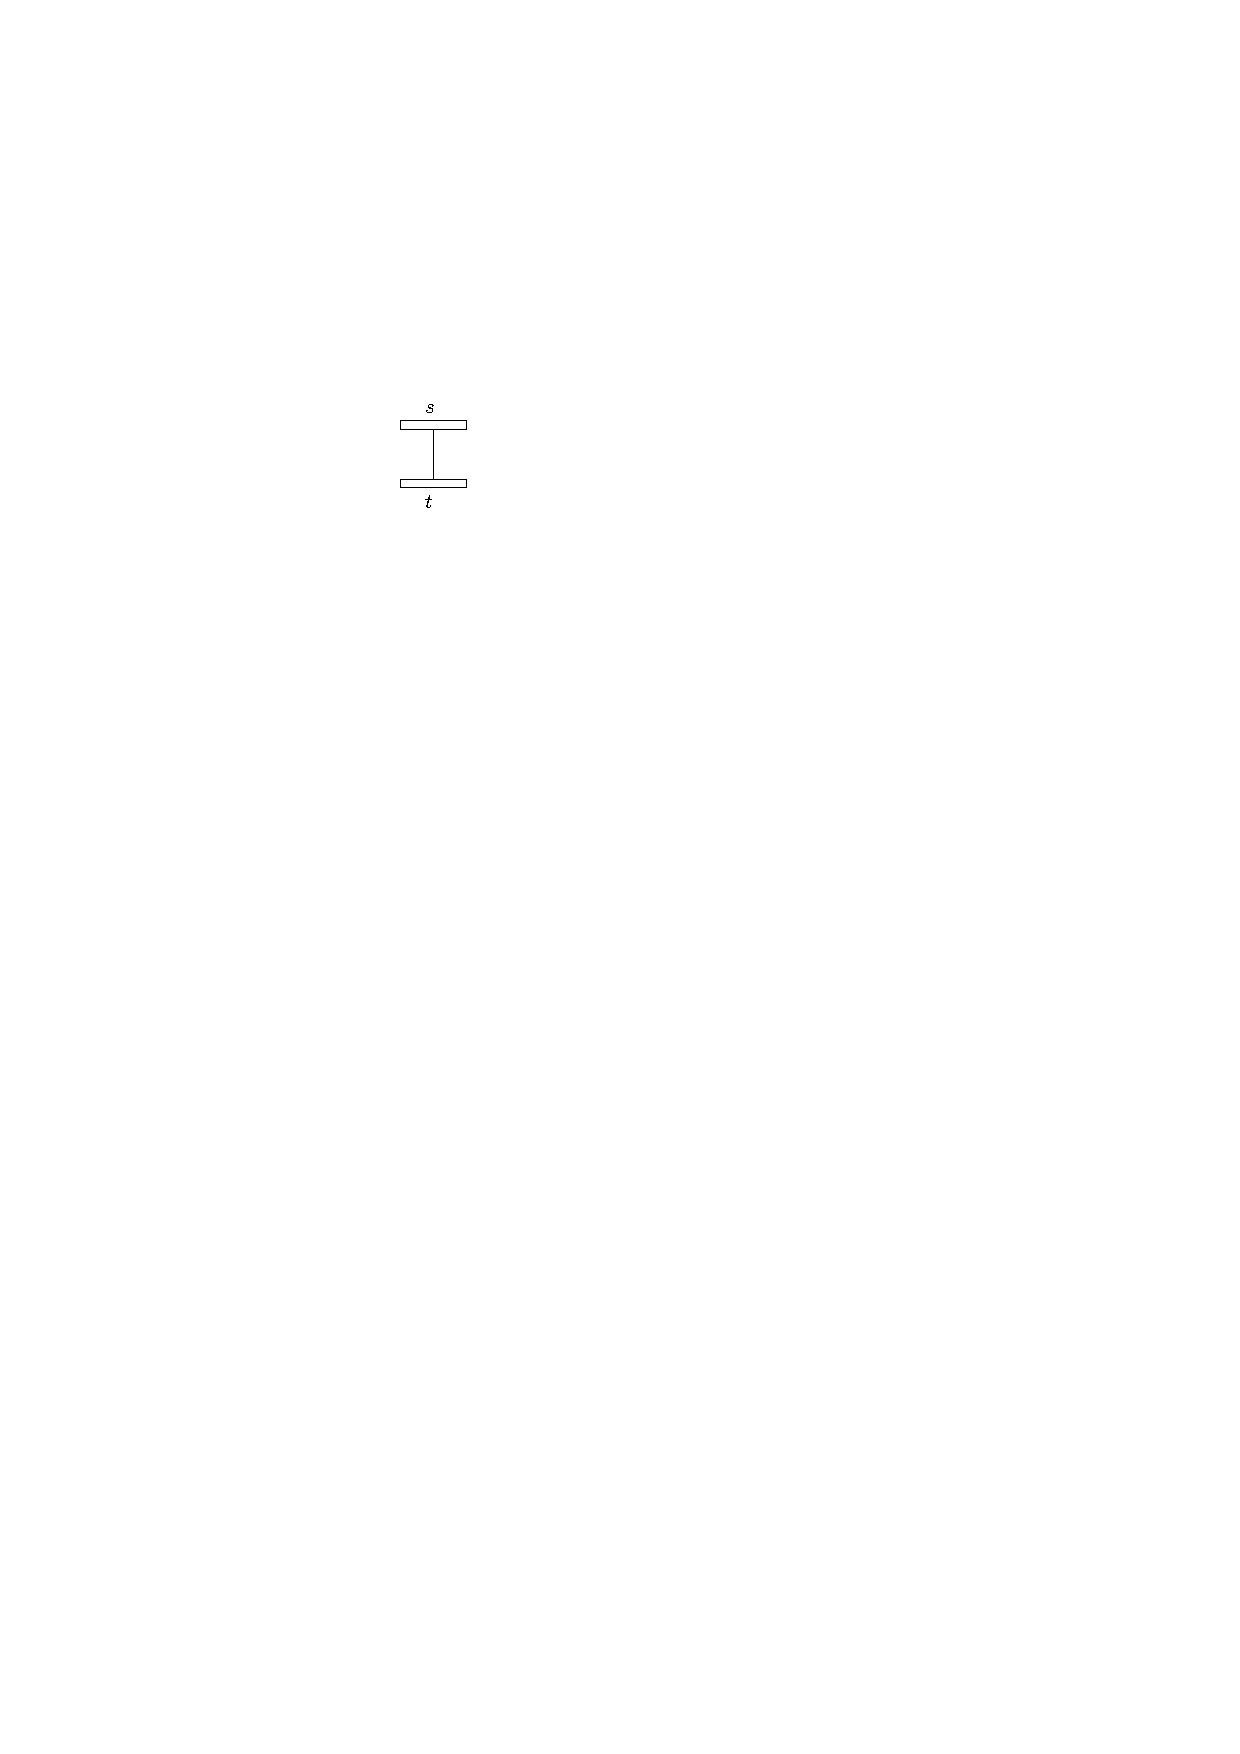
\includegraphics[width=0.4\textwidth,page=1]{drawings/2-trees.pdf}
		\end{subfigure}
		\caption{Basecase }\label{im:SP_basecase}
	\end{figure}
	\item[Height] The height of a drawing can be increased in order to preserve the invariant. 
		\begin{figure}[H]
	\centering
	\begin{subfigure}{0.4\linewidth}
		\centering
		\includegraphics[width=0.7\textwidth,page=2]{drawings/2-trees.pdf}
		\caption{}
	\end{subfigure}
	\begin{subfigure}{0.4\linewidth}
	\centering
	\includegraphics[width=0.6\textwidth,page=3]{drawings/2-trees.pdf}
	\caption{}
\end{subfigure}
	\caption{Terminal release so that $s,t$ span the bounding box (b)}\label{im:SP_terminal-release}
\end{figure}
	\item[Inductive step] This step is for $m>1$ edges and holds two major cases: a parallel composition and a serial composition. If the composition is a parallel one, then the recursive drawings of the $k$ parallel subgraphs will be of a serial composition and vice versa.

	\begin{itemize}
		\item During the parallel composition, $2\leq k$ subgraphs will first be ordered in their number of edges $(m_i \leq m_{i-1}, i \in[1..k])$ and then recursively drawn. The subgraphs are drawn in serial since the original step is the parallel case. The heights of the subgraph drawings are adjusted and unified with a terminal $s$ and $t$ on top and bottom of the bounding box. The height is bound by $h_p(m)\leq\max\{h(m-1),h\left(\frac{m}{2}\right)+2\}$
		\begin{figure}[H]
			\centering
			\begin{subfigure}{0.7\linewidth}
				\centering
				\includegraphics[width=0.9\textwidth,page=4]{drawings/2-trees.pdf}
			\end{subfigure}
			\caption{Case P}\label{im:SP_CaseP}
		\end{figure}
		\item For the serial composition, two subgraphs $H_a, H_b$ with terminals  $s,x$ and $x,t$ are recursively drawn (in parallel). In a trivial case, one of the subgraphs is an edge and $h(m)\leq h(m-1)$. Note, that $x,t$ is an edge of $H_b$ since the original graph is a maximal series-parallel one. There are two outcomes of serial placement. Either, the boxes for $x$ and $t$ share the same row on the bottom of the bounding box, being connected horizontally, or $x$ lies in an interior row and is connected to $t$ vertically. A precomputed index $L$ determines, which case of serial composition holds (\cite{DBLP:journals/dcg/Biedl11}, Lemma 3.3, Page 11).
\begin{figure}[H]
			\centering
			\begin{subfigure}{0.4\linewidth}
				\centering
				\includegraphics[width=0.9\textwidth,page=5]{drawings/2-trees.pdf}
			\end{subfigure}
			\caption{Case S1}\label{im:SP_CaseS1}
		\end{figure}
		\begin{figure}[H]
	\centering
	\begin{subfigure}{0.8\linewidth}
		\centering
		\includegraphics[width=\textwidth,page=6]{drawings/2-trees.pdf}
		\caption{}
	\end{subfigure}
	\begin{subfigure}{0.8\linewidth}
		\centering
		\includegraphics[width=\textwidth,page=7]{drawings/2-trees.pdf}
		\caption{}
	\end{subfigure}
	\caption{Cases S2(a) and S2(b)}\label{im:SP_CaseS2ab}
\end{figure}
		The height is bound by:
		\begin{align}
			h_{S2a}(m)&\leq \max\{h(m-1),h\left(\frac{m}{2}\right)+L\}\\
			h_{S2b}(m)&\leq \max\{h(m_a)+2,h\left(\frac{m_a}{2}\right)+L\}+h(m_L)+1
		\end{align}
	\end{itemize}
	\item[Output] The resulting drawing is a flat orthogonal box drawing. There are no additional columns for the vertices, every vertex contains an incident vertical edge in the base case. Since no bend is created at any time, the box drawing is in fact a flat visibility representation. It was shown that the height of the drawing is bound by $\mathcal{O}(\sqrt{n})$ and there are maximal as many columns as there are edges. The resulting drawing is in area $\mathcal{O(n^{\frac{3}{2}})}$.
	\item[Runtime] Since in this recursive algorithm every edge is touched exactly once, the total runtime lies in $\mathcal{O}(m+n)$.[\cite{DBLP:journals/dcg/Biedl11}: Page 10]
\end{description}

In the resulting flat orthogonal drawing without any bends / visibility representation with $\mathcal{O}(n)$ width and $\mathcal{O}(\sqrt{n})$ height, the longest edge lies in $\mathcal{O}(n)$ since edges are horizontal or vertical line segments. The shortest edge values 2 \UL~in the base case.
\bigskip\\
To transfer a flat orthogonal drawing to a polyline drawing, empty grid lines are inserted until every edge length is at of least two. For a box of a vertex $v$, replaced the box by an arbitrary grid point and insert a bend for each edge connected to $v$ for rerouting. For each vertex, a bend might be inserted, resulting in a polyline drawing with up to two bends per edge.
\begin{lemma}
	Every maximal series-parallel graph admits a polyline drawing with two bends per edge and an edge-length ratio of $\mathcal{O}(n + \sqrt{n}) = \mathcal{O}(n)$.
\end{lemma}
\begin{proof}
	In the transition, every box of vertex in the orthogonal box drawing is substituted with a dot on the grid, therefore two bends per edge. A vertex box has width at most $\mathcal{O}(n)$, like the total width. The longest vertical edge lies in $\mathcal{O}(\sqrt{n})$, is horizontally rerouted with a line segment in $\mathcal{O}(n)$. The shortest edge stays in $\mathcal{O}(1)$, therefore the total edge-length ratio lies in $\mathcal{O}(n)$.
\end{proof}
In the next section, a modification of the three cases of the recursion will lead to a constant ratio while the area consumption is slightly increased.
\subsection{The modification}
The modification alters line segments for every case of recursion while maintaining the invariant. All line segments will be longer than a variable noted $l_{\min}$. The behaviour of the height for every recursion is of interest.
\begin{description}
	\item[Invariant] The invariant will still hold for every case of recursion.
	\item[Base case] the base case is the edge $(s,t)$. Simply put $s$ over $t$ and the invariant holds. It must hold that $h(1) \leq l_{\min}$ in order to validate a small edge-length ratio.
\begin{figure}[H]
	\centering
	\begin{subfigure}{0.2\linewidth}
		\centering
		\includegraphics[width=0.9\textwidth,page=8]{drawings/2-trees.pdf}
	\end{subfigure}
	\caption{Case P}\label{im:SPm_basecase}
\end{figure}
	\item[Height] The height of a drawing can be increased in order to preserve the invariant. But, the height increase must value at least $l_{\min}$. Otherwise, an edge of length one could be placed below $s$ or above $t$.
\begin{figure}[H]
	\centering
	\begin{subfigure}{0.4\linewidth}
		\centering
		\includegraphics[width=0.7\textwidth,page=9]{drawings/2-trees.pdf}
	\end{subfigure}
	\caption{The terminal release must insert edges of length at least $l_{\min}$}\label{im:SPm_terminal-release}
\end{figure}
	\item[Inductive step] 
	\begin{itemize}
		\item During the parallel composition, $2\leq k$ subgraphs will first be ordered in their number of edges $(m_i \leq m_{i-1}, i \in[1..k])$ and then recursively drawn. The height is bound by $h_p(m)\leq\max\{h(m-1),h\left(\frac{m}{2}\right)+2\cdot l_{\min}+2\}$, since the terminal releases must still maintaing a minimum length of $l_{\min}$.
	\begin{figure}[H]
		\centering
		\begin{subfigure}{0.4\linewidth}
			\centering
			\includegraphics[width=0.7\textwidth,page=10]{drawings/2-trees.pdf}
		\end{subfigure}
		\caption{Case P in the modification. Where the orange line segments are placed, there are potential terminal releases which increase the height at least by $l_{\min}$}\label{im:SPm_caseP}
	\end{figure}	
		\item For the serial composition, two subgraphs $H_a, H_b$ with terminals  $s,x$ and $x,t$ are recursively drawn (in parallel). In a trivial case, one of the subgraphs is an edge and $h(m)\leq h(m-1)$. Here, the vertical line segment gets a bend to be elongated up to $2\cdot h_{S_1}(m)$. In the case S2a, the bend is inserted in the same way. Note, that possible terminal releases add the minimum length twice to $h_{S2a}(m)$. In the case S2b, no bend is introduced, but there are up to four terminal release induced height increases by $l_{\min}$.
\begin{figure}[H]
	\centering
	\begin{subfigure}{0.4\linewidth}
		\centering
		\includegraphics[width=0.7\textwidth,page=11]{drawings/2-trees.pdf}
	\end{subfigure}
	\caption{Case S1 gets a bend so the minimum length restriction still holds}\label{im:SPm_S1}
\end{figure}
\begin{figure}[H]
	\centering
	\begin{subfigure}{0.7\linewidth}
		\centering
		\includegraphics[width=\textwidth,page=12]{drawings/2-trees.pdf}
		\caption{}
	\end{subfigure}
	\begin{subfigure}{0.7\linewidth}
	\centering
	\includegraphics[width=\textwidth,page=13]{drawings/2-trees.pdf}
	\caption{}
\end{subfigure}
	\caption{Cases S2a and b also get a bend where necessary and inherit potential terminal release height increases by $l_{\min}$, analoguosly to case P in Figure \ref{im:SPm_caseP}}\label{im:SPm_S2ab}
\end{figure}
		The height is bound by:
		\begin{align}
			h_{S2a}(m)&\leq \max\{h(m-1),h\left(\frac{m}{2}\right)+L+l_{\min}+1\}\\
			h_{S2b}(m)&\leq \max\{h(m_a)+2,h\left(\frac{m_a}{2}\right)+L\}+h(m_L)+1 + 4\cdot l_{\min}+4
		\end{align}
	\end{itemize}
	\item[Output] 
	\item[Runtime] Since in this recursive algorithm every edge is touched exactly once, the total runtime lies in $\mathcal{O}(m+n)$.[\cite{DBLP:journals/dcg/Biedl11}: Page 10]
\end{description}
The resulting drawing is a box drawing with up to one bend per edge. It was shown that the height of the drawing is bound by $\mathcal{O}(\sqrt{n}+l_{\min})$. As before, in order to get a poly-line drawing, insert empty grid lines so that every edge is at least of length $l_{\min}$ and substitute a box with a bend and a suiting line segment. The resulting poly-line drawing will inherit three bends per edge and will fit on an area of $\mathcal{O}(n)\times \mathcal{O}(\sqrt{n}+l_{\min})$.\bigskip\\

\begin{theorem}\label{theorem:2-tree_result}
	Every 2-tree $G$ admits a poly-line drawing on $\mathcal{O}(n^2)$ area with an edge-length ratio of $\mathcal{O}(1)$, using three bends per edge.
\end{theorem}
\begin{proof}
	Let $l_{\min} := n$. After applying the modifiend drawing algorithm by Biedl, the resulting box drawing inherits a height of $\mathcal{O}(\sqrt{n}+n) = \mathcal{O}(n)$. The width still remains at $\mathcal{O}(n)$. There is up to one bend per edge. After the transition to a poly-line drawing, boxes are substituted with line segments, bends and the corresponding vertex and the area bound still holds. To calculate an upper bound for the length of the longest possible edge, we recall that a 2-tree can have at most $2n-3$ edges and the following bounds hold for the resulting drawing:
	\begin{itemize}
		\item Analogously to the original upper bound, after the modification the height is bound by:
		\begin{align}
			h_{mod}(m) \leq 10\cdot\sqrt{2n-3}+4n+4
		\end{align}
	\item An edge corresponds to up to three columns after the modification since one bend is introduced for vertical aligned edges. The amount of the original width is therefore tripled and can be bound by $6n-9$. 
	\end{itemize}
For the ratio, it holds:
\begin{align}
	r = \frac{l_{\max}}{l_{\min}} \leq \frac{h_{mod}(m)+2\cdot w_{mod}(m)}{n} \leq 26 -\frac{14}{n} \leq 26\in\mathcal{O}(1)
\end{align}
\end{proof}